% Cover letter: Data Engineer, Wearables (Job #176270, Topeka, Kansas), Colgate-Palmolive
% CV: Sections/cv_data_engineer.tex -> cv_gen/cv_giovanni_tauro-colgate_palmolive.pdf
\documentclass[11pt,a4paper,sans]{moderncv}
% Shared preamble and header for the cover letters.
% One main file per application: cl_<company>.tex, built to
% cv_gen/coverletter_giovanni_tauro-<company>.pdf next to cv_giovanni_tauro-<company>.pdf.
% Paths (cl_gen/..., Pictures/...) are relative to the project root, as in the CV (see .latexmkrc).

\moderncvstyle{classic}
\moderncvcolor{blue}

\usepackage[scale=0.80]{geometry}
\setlength{\footskip}{136.00005pt}

\usepackage{fontawesome5}
% hyperref is loaded by moderncv itself; loading it here causes an option clash
\usepackage{xcolor}
\usepackage{graphicx}
\ifxetexorluatex
  \usepackage{fontspec}
  \usepackage{unicode-math}
  \defaultfontfeatures{Ligatures=TeX}
  \setmainfont{Latin Modern Roman}
  \setsansfont{Latin Modern Sans}
  \setmonofont{Latin Modern Mono}
  \setmathfont{Latin Modern Math}
\else
  \usepackage[T1]{fontenc}
  \usepackage{lmodern}
\fi

\usepackage[english]{babel}

% used for the PDF title and the letter closing; the visible header is \clheader below
\name{Giovanni}{Tauro}

% Header: #1 = headline under the name (same as the headline of the matching CV)
\newcommand{\clheader}[1]{%
\noindent
\begin{minipage}[c]{0.74\textwidth}
    {\Huge \textbf{Giovanni Tauro}}\\[-0.2em]
    {\small #1}\\[0.3em]

    \footnotesize
    \faMapMarker*~
    \href{https://www.google.com/maps/search/?api=1&query=Lecco+23900+Italy}
    {\color{blue}Bari-Lecco, Italy}
    \quad
    \faPhone*~
    \href{https://wa.me/393279437161}
    {\color{blue}+39 3279437161}
    \quad
    \faEnvelope~
    \href{mailto:giovanni.taurodi@gmail.com}
    {\color{blue}giovanni.taurodi@gmail.com}
    \\[-0.1em]

    \faLinkedin~
    \href{https://www.linkedin.com/in/giovanni-tauro-gt/}
    {\color{blue}LinkedIn}
    \quad
    \faGithub~
    \href{https://github.com/jotades}
    {\color{blue}GitHub}
    \quad
    \faGraduationCap~
    \href{https://scholar.google.com/citations?user=BS0aVGgAAAAJ&hl=it}
    {\color{blue}Scholar}
    \quad
    \faFilePdf~
    \href{https://www.notion.so/Giovanni-Tauro-2a7901d92f3a800b892af425c5875c6a}
    {\color{blue}Portfolio}
    \quad
    \faCubes~
    \href{https://grabcad.com/giovanni.tauro-3}
    {\color{blue}GrabCAD}

\end{minipage}
\hfill
\begin{minipage}[c]{0.18\textwidth}
    \raggedleft
    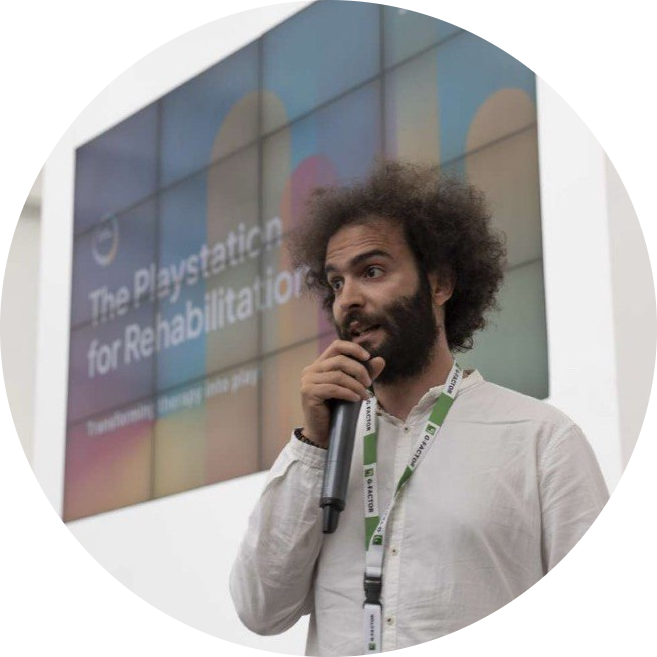
\includegraphics[width=2.8cm]{Pictures/Giovanni_pitch}
\end{minipage}
\vspace{0.1em}
}

\makeatletter
% the sender details are already in \clheader, so skip moderncv's own block
\@detailsfalse
% closing phrase, signature, name
\renewcommand*{\makeletterclosing}{%
  \@closing\\[0.6em]%
  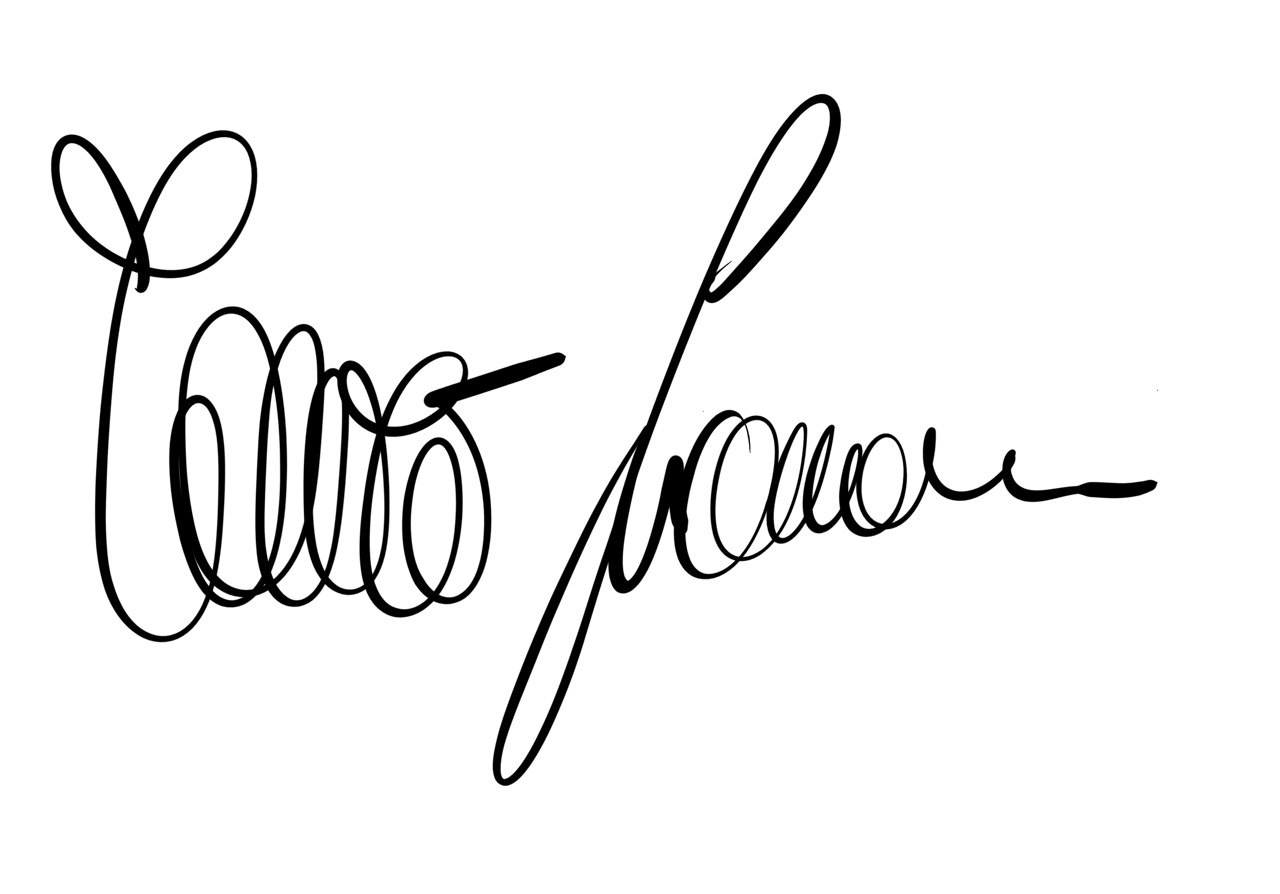
\includegraphics[height=1.2cm]{Pictures/sign_gt.jpg}\\[0.2em]%
  {\bfseries\@firstname~\@lastname}}
\makeatother


\begin{document}

\clheader{R\&D Engineer, PhD Candidate | Wearable Sensor Data \& IoT}

\recipient{Talent Acquisition Team}{Colgate-Palmolive Company}
\opening{Dear Hiring Team,}
\closing{Sincerely,}
\makelettertitle

I am applying for the Data Engineer, Wearables position (Job Number 176270). I am an R\&D engineer and PhD candidate with more than five years at CNR-STIIMA, the Italian National Research Council, building wearable and IoT sensing systems for health research. Most of that work is turning raw sensor signals into datasets that researchers can trust.

For my PhD project, OmniTrack, I built the data pipeline end to end. Wearable tags send ultra-wideband ranging and IMU time series, ROS 2 nodes estimate each position, and every session is logged in MongoDB. On top of this I developed OmniAnalytics, a Python backend (pandas, FastAPI) with a React dashboard, which turns the raw recordings of a study with 16 blind participants into trial metrics such as route similarity (dynamic time warping, Fr\'echet distance), speed and target discovery.

I designed it so that results can be traced back to their source. Raw recordings are never modified: corrections for sensor gaps, exclusions and annotations are stored separately, and the code is versioned in Git.

I am also used to the setting around the data. PhiCube, the rehabilitation device I co-invented, is deployed in Italian clinics and is in two ongoing multicentre studies with 134 patients, and I defined its requirements together with clinicians. As Head of Product and co-founder of Rehabilia Technologies I set priorities and work with engineering, design and clinical partners, which has taught me to explain technical choices to people who are not engineers.

My sensor data so far comes from people rather than companion animals, and I have not yet used BigQuery, Snowflake or Airflow. I have built by hand the stages they serve, from ingestion and cleaning to storage and analysis, and I would expect to become productive with them quickly.

I would welcome the chance to discuss the role further.

\makeletterclosing

\end{document}
